\appendix


\chapter{Script}

\section{Operativi}
\subsection{Script per la lettura dei valori misurati da Accelerometro e Giroscopio tramite I2C}
\label{scriptXLGRead}
Di seguito si riporta il codice utilizzato per leggere i dati misurati dall'accelerometro e dal giroscpio utilizzando un canale I2C in fast-mode.\\
\noindent\rule{14.1cm}{0.4pt}
\begin{lstlisting}[language=C]
LSM9DS1_XLG_READ LSM9DS1_Read_XLG(MFX_input_t *data_in, int samples)
{
	int16_t pData[6]={0,0,0,0,0,0};
	int16_t data=0;
	int8_t regadd;
	int i,j,k;
	float divisor=1000;
	float sensitivityXL= (float) LSM9DS1_get_Sens_XL();
	float sensitivityG= (float) LSM9DS1_get_Sens_G();

	uint8_t hi;
	uint8_t lo;

	/* Read output registers from LSM9DS1_OUT_X_L_G to LSM9DS1_OUT_Z_XL. */
	for (i = 0; i < samples; i++ )
	{
		regadd=LSM9DS1_OUT_X_L_G;

		//read Gyroscope output
		for (j = 0; j < 3; j++ )
		{
			if( !I2C_ReadData(LSM9DS1_I2C_BADD, regadd, &lo,1))
			{
				return 0;
			}
			regadd++;
			if( !I2C_ReadData(LSM9DS1_I2C_BADD,regadd, &hi,1))
			{
				return 0 ;
			}
			regadd++;

			data = ((uint16_t)hi << 8) | (uint16_t)lo;
			pData[j]=data;

		}
		/* Format the data. */
		data_in->gyro[0] =  (pData[0] * sensitivityG )/divisor;
		data_in->gyro[1] =  (pData[1] * sensitivityG )/divisor;
		data_in->gyro[2] = ((pData[2] * sensitivityG )/divisor);

		regadd=LSM9DS1_OUT_X_L_XL;
		//read Accelerometer output
		for (j = 3; j < 6; j++ )
		{
			if( !I2C_ReadData(LSM9DS1_I2C_BADD, regadd, &lo,1))
			{
				return 0;
			}
			regadd++;
			if( !I2C_ReadData(LSM9DS1_I2C_BADD,regadd, &hi,1))
			{
				return 0 ;
			}
			regadd++;

			data = ((uint16_t)hi << 8) | (uint16_t)lo;
			pData[j]=data;

		}
		/* Format the data. */
		data_in->acc[0] =  (pData[3] * sensitivityXL)/divisor;
		data_in->acc[1] =  (pData[4] * sensitivityXL)/divisor;
		data_in->acc[2] = (pData[5] * sensitivityXL)/divisor;
	}
	return 1;
}



\end{lstlisting}

\section{Testing}
\subsection{Script per la stima del tempo di lettura di dati provenienti dall'IMU }
\label{app:stimai2c}
Di seguito si riporta il codice utilizzato per stimare il tempo di lettura di dati provenienti dall'unità di misura inerziale utilizzando un canale I2C in fast-mode.\\
\noindent\rule{14.1cm}{0.4pt}
\begin{lstlisting}[language=C]
//Test I2C speed
while(1){
if(id<1000){

	if(!I2C_ReadData(LSM9DS1_I2C_BADD,LSM9DS1_WHO_AM_I,&result,1)){
		if( result == LSM9DS1_WHO_AM_I_VALUE)
				id++;
	}
	else
	{
		lost++;
	}
	
 	if(id==1000){
		t1=HAL_GetTick()-t0;
		HAL_Delay(2);
		snprintf(data, 10, "%Lu",t1);
		CDC_Transmit_FS((uint8_t *)data,strlen(data));
	}
}



\end{lstlisting}


\subsection{Script per la stima del tempo di trasmissione di dati al modulo App}
\label{app:stimausb}
Di seguito si riporta il codice utilizzato per stimare il tempo di trasmissione sul canale USB utilizzato nella classe CDC.\\
\noindent\rule{14.1cm}{0.4pt}

\begin{lstlisting}[language=C]
 //Test usb CDC speed
while(1)
{
	snprintf(data, 10, "%d|%d\n",id,lost);
	if(id<1000){
		if(CDC_Transmit_FS((uint8_t *)data,strlen(data))== USBD_OK)
		{
			id++;
		}
		else{
			lost++;
		}

	if(id==1000){
		t1=HAL_GetTick()-t0;
		snprintf(data, 10, "%Lu\n",t1);
		CDC_Transmit_FS((uint8_t *)data,strlen(data));
	}
	
}



\end{lstlisting}


\chapter{Filtro di Kalman}
\label{appendixKalman}
In questa seziona si riporta l'appendice riguardante la teoria e i fondamenti del filtro di Kalman \cite{trackingThesis}.\\
Il filtro di Kalman può essere utilizzato per stimare lo stato passato, presente e futuro di un sistema nel quale le variabile di input e output non sono completamente note in quanto affette da rumore.\\
Il filtro permette di ottenere una prima \textit{stima a priori}. Nell'ambito di questa tesi lo stato è l'assetto e la stima è fatta a partire dai dati del giroscopio. Successivamente la stima a \textit{priori} viene raffinata usando l'accelerometro ed eventualmente anche il magnetometro, per ottenere quella che viene chiamata \textit{stima a posteriori}.
Come è facile capire, è possibile usare il filtro di Kalman in tutti i casi in cui è necessario fondere dati provenienti da sorgenti diverse, ottenendo una stima del sistema migliore col crescere dei sensori utilizzati, che sono tuttavia affetti da rumore.

\section{Descrizione teorica del filtro di Kalman}
\label{filtroKalmanLineare}
E' possibile descrive un sistema a tempo discreto con un'equazione stocastica lineare del tipo:
\begin{equation}
x_k = Ax_{k-1} + B u_k + w_{k-1}
\end{equation}
Dove $x_k \in \Re^n$ è il vettore che descrive lo stato del sistema, $u_k$ è il vettore di dimensione $l$ con le variabili d'ingresso del sistema, $A$ è una matrice $n \times n$ che descrive l'evoluzione del sistema senza input, $B$ è la matrice $n \times l$ che lega l'evoluzione del sistema con il vettore d'ingressi $u_k$ ed infine $w_{k-1}$ è il vettore contenente i rumori del processo.\\
Le variabili di output sono descritte invece dalla seguente equazione:
\begin{equation}
z_k = Hx_k + v_k
\end{equation}
Dove $z_k$ è il vettore con le variabili di output, $H$ è la matrice che lega lo stato del sistema con l'output e $v_k$ è il vettore che descrive la misura del rumore.
Si deve assumere che il processo e la misura del rumore siano indipendenti, bianchi e con una distribuzione Gaussiana:
\begin{equation}
p(w) \sim N(0,Q)
\end{equation}

\begin{equation}
p(v) \sim N(0,R)
\end{equation}

Le due distribuzioni hanno una media pari a zero e una covarianza descritta dalla matrice Q e R. Generalmente, le matrici $Q$ e $R$ possono variare ad ogni iterazione del filtro, ma per semplicità nell'ambito di questa tesi sono considerate costanti.\\
Si definisce $\hat{x}_k^-$ la stima a \textit{priori} dello stato del sistema, mentre con $\hat{x}_k$ la stima a \textit{posteriori}. Se $x_k$ è lo stato reale del sistema, è possibile definire l'errore a \textit{priori} e a \textit{posteriori} della stima del sistema:
\begin{equation}
e_k^- \equiv x_k - \hat{x}_k^-
\end{equation}

\begin{equation}
e_k \equiv x_k - \hat{x}_k
\end{equation}

Poiché questo sistema è caratterizzato da un rumore descritto tramite variabili statistiche, è possibile caratterizza statisticamente anche l'errore della stima dello stato del sistema. In particolare, la covarianza dell'errore nella stima a \textit{priori} e a \textit{posteriori} è rispettivamente:
\begin{equation}
P_k^- = E[e_k^-e_k^{-T}]
\end{equation}
\begin{equation}
\label{pk}
P_k = E[e_ke_k^{T}]
\end{equation}
La stima a \textit{posteriori} dello stato del sistema è data dalla seguente equazione:
\begin{equation}
\label{eq:stimaPoste}
\hat{x}_k= \hat{x}_k^- + K ( z_k - H \hat{x}_k^-)
\end{equation}
Dove si lega la stima a \textit{priori} con quella che viene chiamata misura innovativa o residuo. Questa è la differenza tra l'attuale misura $z_k$ e la misura predetta tramite $H\hat{x}_k^-$.\\
Da \ref{eq:stimaPoste} si può notare che la misura a \textit{priori} $\hat{x}_k^-$ è corretta con una quantità data dalla moltiplicazione del residuo con la matrice $K$ di dimensione $n \times m$. Questa matrice è detta \textbf{matrice del guadagno di Kalman} ed è calcolata per minimizzare $P_k^-$, la matrice di covarianza dell'errore a \textit{priori}, al fine di ottenere la stima ottima dello stato del sistema.\\
Sostituendo \ref{eq:stimaPoste} alla definizione di $e_k$ e in \ref{pk}, derivando rispetto a $K$ e risolvendo per trovare il minimo, si può scrivere la seguente equazione per calcolare la matrice del guadagno di Kalman:
\begin{equation}
K_k = P_k^{-1} H^T ( HP_k^- H^T + R)^{-1} = \dfrac{P_k^{-1}H^T}{HP_k^-H^T + R}
\end{equation}
Si noti come anche la matrice $K$ potrebbe cambiare ad ogni iterazione del filtro. Si possono fare delle considerazione interessanti per capire meglio il filtro di Kalman. Infatti, se la covarianza dell'errore $R$ è vicina allo zero, il filtro pesa più la misura $z_k$ rispetto alla stima a \textit{priori} $\hat{x}_k^-$ per ricostruire lo stato del sistema. In questo caso:
\begin{equation}
\lim\limits_{R\rightarrow0}K_k=H^{-1};  \lim\limits_{R\rightarrow0}\hat{x}_k= H^{-1}z_k
\end{equation}
Nel caso opposto che la matrice di covarianza dell'errore della stima a \textit{priori} sia vicina allo zero, la matrice $K$ tende anch'essa a zero. In questo caso, il residuo conta meno per la stima dello stato a \textit{posteriori}, che tende ad essere uguale alla stima a \textit{priori}:
\begin{equation}
\lim\limits_{P_k^-\rightarrow0}K_k=0;  \lim\limits_{P_k^-\rightarrow0}\hat{x}_k=  \hat{x}_k^-
\end{equation}
Si può concludere che, se il processo e la misura del rumore sono Gaussiani, bianchi e indipendenti, allora la stima del sistema $x_k$ è una variabile Gaussiana con media pari a $\hat{x}_k$ e covarianza $P_k$.

\section{L'algoritmo del filtro di Kalman discreto}

Come si è appena visto, il filtro di Kalman prova a stimare lo stato di un sistema con qualcosa di simile ad un feedback di controllo. L'equazioni del filtro sono divise in due differenti tipi: \textbf{l'equazioni di update} dello stato, anche chiamate equazioni di predizione, che aggiornano la sitma a \textit{priori} dello stato del sistema e \textbf{l'equazioni di misura} che sono responsabili di correggere il feedback e la stima a \textit{posteriori}.\\
L'equazioni di predizione sono:
\begin{equation}
\label{eq:xkc}
x_k^- = A\hat{x}_{k-1} + B u_k
\end{equation}

\begin{equation}
\label{eq:pkc}
P_k^- = AP_{k-1}A^T + Q
\end{equation}
Si può notare che la stima a \textit{priori} di $x_k^-$ è fatta a partire dalla stima a posteriori dello stato del sistema ottenuta nell'iterazione precedente $k-1$.\\
La matrice di covarianza dell'errore dello stato, stimato a \textit{priori}, è anch'essa calcolata a partire da quella calcolata a posteriori nell'iterazione precedente e poi sommata con la matrice $Q$, che è la covarianza del rumore del processo.
L'equazioni di misura sono:
\begin{equation}
\label{eq:kk}
K_k = P_k^-H^T (HP_k^- HT + R)^{-1}
\end{equation}

\begin{equation}
\label{eq:xk}
\hat{x}_k = \hat{x}_k^- + K(z_k - H\hat{x}_k^-)
\end{equation}

\begin{equation}
\label{eq:pk}
P_k = (I - K_k H) P_k^-
\end{equation}

Nel primo step la matrice del guadagno di Kalman $K_k$ è aggiornata. Questo è necessario per misurare l'output del sistema $z_k$ e per calcolare la stima a \textit{posteriori} $\hat{x}_k$. Nell'ultimo step, si calcola, a \textit{posteriori}, la matrice di covarianza dell'errore $P_k$. \\
Per ogni iterazione del filtro, l'equazione \ref{eq:xkc} e  \ref{eq:pkc} sono utilizzate per calcolare la stima a \textit{priori} dello stato allo step $k$, quindi si utilizzano \ref{eq:kk}, \ref{eq:xk} e \ref{eq:pk} per calcolare la stima a \textit{posteriori}. Allo step successivo $k+1$ viene ripetuto quanto appena detto utilizzando la stima a posteriori calcolata nell'iterazione precedente, come mostrato nella figura seguente:
\begin{figure}[H]  
	\centering 
	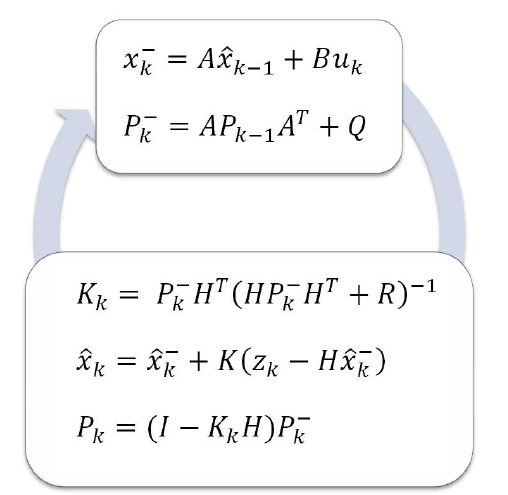
\includegraphics[scale=0.8]{kalman/kalmanfilter.png}
	\caption{Rappresentazione dell'algoritmo di Kalman per un sistema tempo discreto}
	\label{fig:kalmanfilter}
\end{figure}
E' ora necessario vedere come inizializzare il filtro e quali valori bisogna stimare e misurare. Per prima cosa, il sistema deve essere modellato, quindi è necessario stimare le matrici $A$ e $B$ che descrivo l'evoluzione del sistema e la matrice $H$ che lega lo stato del sistema con la misura dell'output. E' necessario inoltre misurare o calcolare la matrice $R$ che, come detto, rappresenta la covarianza dell'errore delle misure. \\
La matrice $Q$ non è sempre direttamente misurabile, questo perché lo stato del sistema di solito non può essere misurato.\\
All'inizio, il filtro deve essere inizializzato con qualche valore di $\hat{x}_0$ e $P_0$. Questi valori non sono veramente importanti in quanto il filtro è ben implementato, dopo un certo numero di iterazioni lo stato del sistema convergerà alla stima corretta indipendentemente dal valore $\hat{x}_0$ scelto. Tuttavia una scelta corretta va ad inficiare sulla lunghezza e sull'intensità di questo transitorio iniziale.\\
Una considerazione finale: se la matrice $Q$ e $R$ sono costanti, dopo la prima iterazione del filtro anche i valori $P_k$ e $K_k$ si stabilizzeranno a valori costanti. In questo caso, questi valori possono essere precalcolati durante la fase di settaggio e memorizzati.

\section{Il filtro di Kalman esteso}
Si è visto precedentemente, come funziona il filtro di Kalman e come sia possibile implementarlo a partire da equazioni differenziali lineari stocastiche che descrivo l'evoluzione del sistema. Il problema è che tutte le considerazioni fatte valgono solo per i sistemi lineari, ma la maggior parte delle applicazioni reali riguardano sistemi non lineari e il lavoro di questa tesi non fa eccezione.\\
Si deve considerare una nuova versione del filtro di Kalman, il \textbf{filtro di Kalman estesto} (EKF). Questa versione funziona con sistemi non lineare e usa li linearizza attorno al punt di lavoro attraverso una matrice Jacobbiana.\\
In questo caso il sistema è descritto da un'equazione stocastica non lineare:
\begin{equation}
x_k = f(x_{k-1},u_k,w_{k-1})
\end{equation}

\begin{equation}
z_k = h(x_k,v_k)
\end{equation}

I termini hanno gli stessi significati della versione lineare del filtro \ref{filtroKalmanLineare} con la differenza che ora appaiono all'interno di un'equazione non lineare.\\
Deve essere fatto presente che, sicché si tratta di un'equazione non lineare e nonostante  $w_k$ e $v_k$ siano rumori bianchi Gaussiani, il rumore generato non è Gaussiano. Tuttavia grazie alla linearizzazione intorno al punto di lavoro, questo può essere considerato come tale.\\
Di solito, è possibile approssimare lo stato e le misure considerando il rumore uguale a zero:
\begin{equation}
\label{eq:nonL1}
\tilde{x}_k = f(x_{k-1},u_k,0)
\end{equation}
\begin{equation}
\label{eq:nonL2}
\tilde{z}_k = h(\tilde{x}_k,0)
\end{equation}
Per stimare il sistema descritto da un'equazione non lineare è possibile scrivere due equazioni linearizzate che includono la stima di $\tilde{x}_k$ e $\tilde{z}_k$ viste precedentemente:
\begin{equation}
	x_k \approx \tilde{x}_k + A(x_{k-1} - \hat{x}_{k-1}) + Ww_{k-1}
\end{equation}

\begin{equation}
z_k \approx \tilde{z}_k + H(x_k - \tilde{x}_k) + Vv_k
\end{equation}

Nelle quali, $x_k$ e $z_k$ sono rispettivamente lo stato del sistema e il vettore delle misure, $\tilde{x}_k$ e $\tilde{z}_k$ sono lo stato del sistema e il vettore delle misure approssimate da \ref{eq:nonL1} e \ref{eq:nonL2}, $\hat{x}_k$ è la stima a \textit{posteriori} dello stato all'iterazione $k$, $w_k$ e $v_k$ sono i rumori del processo e delle misure.\\
La matrice Jacobbiana $A$ introdotta è la matrice delle derivate parziali di $f$ rispetto a $x$:
\begin{equation}
A_{[i,j]} = \dfrac{\partial f_{i}}{\partial x_j} ( \hat{x}_k,u_k,0)
\end{equation}

La matrice $W$ è la matrice Jacobbiana delle derivate parziali di $f$ rispetto a $w$:
\begin{equation}
W_{[i,j]} = \dfrac{\partial f_{i}}{\partial w_j} ( \hat{x}_k,u_k,0)
\end{equation}

La matrice $H$ è la matrice Jacobbiana delle derivate parziali di $h$ rispetto ad $x$:
\begin{equation}
H_{[i,j]} = \dfrac{\partial h_{i}}{\partial x_j} ( \tilde{x}_k,0)
\end{equation}

La matrice $V$ è la matrice Jacobbiana delle derivare parziali di $h$ rispetto a $v$:

\begin{equation}
V_{[i,j]} = \dfrac{\partial h_{i}}{\partial v_j} ( \tilde{x}_k,0)
\end{equation}

Ancora una volta si deve sottolineare che le matrici sopracitate potrebbero cambiare ad ogni iterazione del filtro. A questo punto si applicano le notazioni introdotte per l'errore durante la stima dello stato e delle misure approssimate:
\begin{equation}
\label{e_xk}
\tilde{e}_{x_k} \equiv x_k - \tilde{x}_k
\end{equation}

\begin{equation}
\label{ezk_nl}
\tilde{e}_{z_k} \equiv z_k - \tilde{z}_k
\end{equation}

Le precedenti equazioni possono essere approssimate nel seguente modo:

\begin{equation}
\tilde{e}_{x_k} \approx A(x_{k-1} - \hat{x}_{k-1}) + \epsilon_k
\end{equation}

\begin{equation}
\tilde{e}_{z_k} \approx H \tilde{e}_{x_k} + \eta_k
\end{equation}

Ora due nuove variabili casuali e indipendenti sono state introdotte. Queste hanno media pari a zero e la covarianza dell'errore è data dalle matrice $WQW^T$ e $VRV^T$, con $Q$ e $R$ matrici di covarianza dell'errore del processo e della misura rispettivamente.\\
Queste equazione derivate sono lineari e simili a quelle che descrivono l'evoluzione del sistema lineare. Quindi si possono applicare ad un secondo ipotetico filtro di Kalman per stimare l'errore $\tilde{e}_{x_k}$. Questa stima può a sua volta essere usata con \ref{e_xk} per ottenere la stima a \textit{posteriori} dello stato del sistema non lineare:
\begin{equation}
\label{xk_nl}
\hat{x}_k = \tilde{x}_k + \hat{e}_k
\end{equation}

La variabile casuale $\tilde{e}_{x_k}$ ha una distribuzione Gaussiana con una media pari a zero e una covarianza dell'errore $E(\tilde{e}_{x_k}\tilde{e}_{x_k}^T )$. Così, se il valore predetto di $\hat{e}_k$ è zero, l'equazione usata per stimarlo si riduce a:
\begin{equation}
\hat{e}_k = K_k \tilde{e}_{z_k}
\end{equation}
Sostituendo questa relazione in \ref{xk_nl} e poi in \ref{ezk_nl} si ottiene:
\begin{equation}
\hat{x}_k = \tilde{x}_k + K_k\tilde{e}_{z_k} =  \tilde{x}_k + K_k (z_k - \tilde{z}_k)
\end{equation}

Da questo risultato si vede che in realtà non è necessario usare un secondo filtro di Kalman perché l'equazione dipende solo da $\tilde{x}_k$ e $\tilde{z}_k$, che sono definite in \ref{eq:nonL1} e \ref{eq:nonL2}, mentre $K_k$ è il guadagno del filtro di Kalman definito in \ref{eq:kk}.\\
In conclusione, l'equazione del filtro di Kalman esteso sono:

\begin{equation}
\tilde{x}_k = x_k^- = f(\hat{x}_{k-1},u_k,0)
\end{equation}

\begin{equation}
P_k^- = A_k P_{k-1}A_k^T + W_k Q_{k-1} W_k^T
\end{equation}

Mentre l'equazioni di correzione sono:

\begin{equation}
K_k = P_k^- H_k^T (H_kP_k^-H_k^T + V_kR_kV_k^T)^{-1}
\end{equation}

\begin{equation}
\hat{x}_k = \hat{x}_k^- + K_k (z_k - h(\hat{x}_k^-,0))
\end{equation}


\begin{equation}
P_k= (I - K_k H_k)P_k^-
\end{equation}

In queste equazioni finali, al fine di essere coerenti con il filtro di Kalman la notazione $\tilde{x}_k$ è stato sostituita da $x_k^-$.\\
Si noti come le operazioni del filtro di Kalman esteso non siano cambiate rispetto al filtro "normale", con equazioni di predizione e correzione simili eseguite ad ogni iterazione. La grande differenza è che ora le matrici $A$ e $H$ più le matrici $W$ e $V$ sono matrici Jacobbiane con derivate parziali delle funzioni non lineari $f$ e $h$. Di solito, queste matrici sono ricalcolate ad ogni iterazione $k$, come mostrato in figura:

\begin{figure}[H]  
	\centering 
	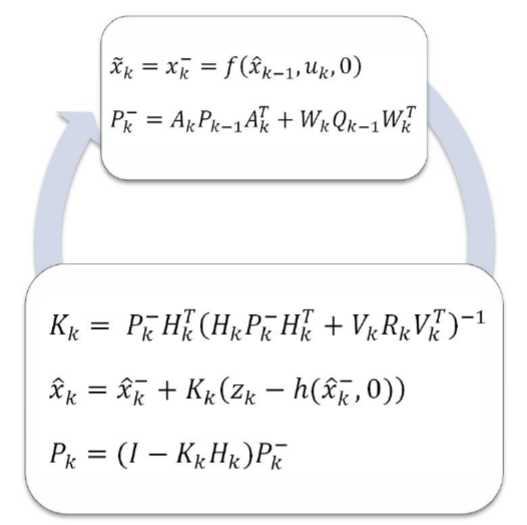
\includegraphics[scale=0.8]{kalman/kalmanfilterNL.png}
	\caption{Rappresentazione dell'algoritmo di Kalman esteso per un sistema tempo discreto non lineare}
	\label{fig:kalmanfilterNL}
\end{figure}







